%! Author = manuel
%! Date = 03.05.21

% compile with pdflatex ./'Report.tex'

% Requirements for this document:

% The submission includes a file in the root of the GitHub repository or zip file (one of Report.md, Report.ipynb, or Report.pdf) that provides a description of the implementation
% The report clearly describes the learning algorithm, along with the chosen hyperparameters. It also describes the model architectures for any neural networks.
% A plot of rewards per episode is included to illustrate that the agent is able to receive an average reward (over 100 episodes) of at least +13. The submission reports the number of episodes needed to solve the environment.
% The submission has concrete future ideas for improving the agent's performance

% Preamble
\documentclass[12pt,a4paper]{article}

% Packages
\usepackage{amsmath}
\usepackage{float}
\usepackage[hscale=0.8,vscale=0.8]{geometry}
\usepackage{amsfonts}
\usepackage{graphicx}

% Document
\begin{document}

    \section{Overview}\label{sec:overview}
    This project demonstrates the use of deep Q-Networks for reinforcement learning.
    Reinforcement learning is a branch of Machine learning where an agent is trained to correctly behave in
    a particular environment.
    The Agent interacts with the environment by choosing some action $a$.
    In response to the action the environment returns a new environment state $s$ and a reward $r$.
    The goal of the agent is to maximize the cumulative reward.
    \\
    In this particular project the agent uses Q-Networks to be able to easily deal with a big set of possible states $S$.
    Q-Network's are deep neural networks that serve as a nonlinear function approximator which are trying to find the best action value function.
    This means the Q-Network tries to estimate the expected sum of future rewards (discounted by $\gamma$) for a given state action pair.
    $$Q_{\pi}(s,a)=\mathbb{E}[\gamma ^{0}R_{1}+\gamma ^{1}R_{2}+\gamma ^{2}R_{3}+...|S_{0}=s, A_{0}=a, \pi]$$
    \\
    Due to the unstable nature of nonlinear functions there are multiple additions of the Deep Q-learning Algorithm to increase the stability.
    This project implements the following two:
    \\\\
    \textbf{Replay Buffer:}
    Use a buffer to store N most recent Experiences ($S, A, R, S'$ tuples).
    Sample n random elements from the buffer at xth every time step and learn from them.
    \\\\
    \textbf{Double DQN:}
    Use two neural networks instead of one to select the best action in order to prevent the algorithm from propagating incidental high rewards received by chance.
    The target network is updated


    \section{Results}\label{sec:results}
    For this Project I tried many runs with different hyper parameters.
    I also tried to change the architecture of the neural networks.
    But as I added more layers/more nodes per layer I noticed that this dramatically decreased the performance of the agent.
    Probably because I would also have to change other hyperparameters such as the learning rate accordingly.
    \\
    One trend I noticed was that each time I increased the number of nodes per layer, the resulting score plot fluctuated much more around the mean.
    This is probably because as the dimensionality of the action value function (characterized by the Q network) increases, the network also looses stability when trained with unchanged hyperparameters.

    \begin{figure}[H]
        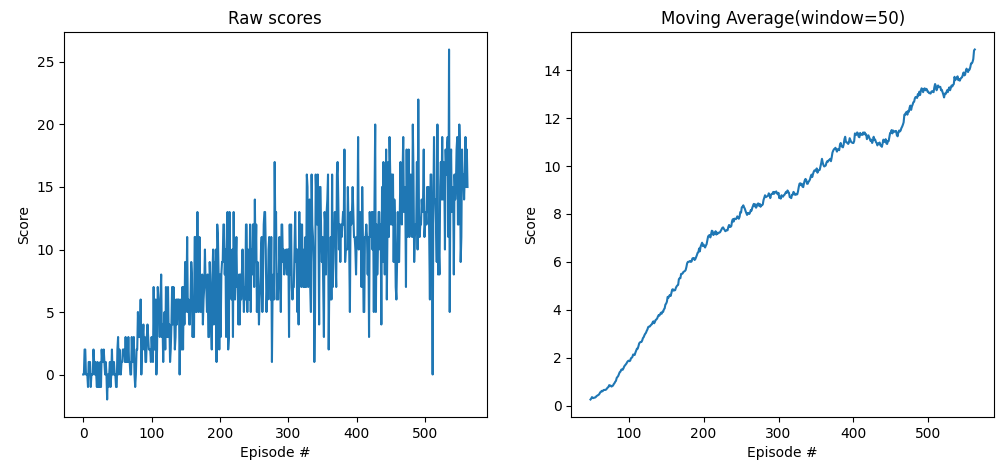
\includegraphics[width=\linewidth]{assets/run-2021-05-06-14-06}
        \caption{Scores that the agent achieved per episode}
        \label{fig:scores}
    \end{figure}


    \section{Ideas for future improvements}\label{sec:ideas}
    One way to improve the Model is always to fine tune the hyper parameters.
    Additionally, it is possible to implement additional algorithms that help to improve and stabilize the DQN algorithm.
    Such additions would be "Dueling DQN", "Distributional DQN" and "Noisy DQN".
    \\\\
    Moreover I noticed that with the given environment states from the unity engine it seems that the agent is not able
    to detect bananas that are very far away.
    Thus, using actual pixel values as input might also improve performance in this particular case.


\end{document}